\documentclass[12pt]{article}

\title{\vspace{-3em}PHYS 167b HW 4}
\author{Michael Cardiff}
\date{\today}

%% science symbols
\usepackage{amsmath}
\usepackage{amssymb}
\usepackage{amsthm}
\usepackage{bm}
\usepackage{cancel}
\usepackage{physics}
\usepackage{siunitx}
\usepackage{slashed}

%% general pretty stuff
% \usepackage[margin=1in]{geometry}
\usepackage{caption}
\usepackage{float}
\usepackage{graphicx}
\usepackage{url}
\usepackage{enumitem}
\usepackage{hyperref}
\usepackage{tikz}
\usepackage{tikz-feynhand}

% setup options
\captionsetup{labelfont=bf}
\graphicspath{ {./figs/} }

% macros
\renewcommand{\bar}{\overline}
\renewcommand{\L}{\mathcal{L}}
\renewcommand{\H}{\mathcal{H}}
\renewcommand{\l}{\ell}
\newcommand{\sla}{\slashed}
\newcommand{\M}{\mathcal{M}}
\newcommand{\mcV}{\mathcal{V}}
\newcommand{\D}{\partial}
\newcommand{\veps}{\varepsilon}
\newcommand{\circled}[1]{\tikz[baseline = (char.base)]{
    \node[shape=circle,draw,inner sep=2pt] (char) {#1};}}

% mdframed environments
\usepackage[framemethod=TikZ]{mdframed}
\mdfsetup{skipabove=\topskip,skipbelow=\topskip}
\mdfdefinestyle{defstyle}{%
  linewidth=1pt,
  frametitlerule=true,
  frametitlebackgroundcolor=gray!40,
  backgroundcolor=gray!20,
  innertopmargin=\topskip}

\mdtheorem[style=defstyle]{definition}{Definition}
\mdtheorem[style=defstyle]{theorem}{Theorem}
\mdtheorem[style=defstyle]{problem}{Problem}[section]

\newenvironment{thebook}
{\begin{mdframed}[style=defstyle,frametitle={From the Book}]}{\end{mdframed}}

\begin{document}
\maketitle

\section{Thomson, Problem 6.2}
\begin{problem}
  Show that the chiral projection operators
  \begin{align*}
    P_R=\frac12(1+\gamma^5)\quad\text{and}\quad P_L=\frac12(1+\gamma^5)
  \end{align*}
  Satisfy the following:
  \begin{align*}
    P_R+P_L=1\quad
    P_R P_R=P_R\quad
    P_L P_L=P_L\quad
    P_L P_R=0
  \end{align*}
\end{problem}
These are all fairly simple to calculate given that $\gamma^5$ squares to the identity:
\begin{align*}
  P_R+P_L&=\frac12(1+\gamma^5+1-\gamma^5)=\frac12(2)=1\\
  P_R P_R&=\frac14(1+\gamma^5)(1+\gamma^5)=
  \frac14(1+\gamma^5+\gamma^5+{(\gamma^5)}^2)=\frac14(2+2\gamma^5)=P_R\\
  P_L P_L&=\frac14(1-\gamma^5)(1-\gamma^5)=
  \frac14(1-\gamma^5-\gamma^5+{(\gamma^5)}^2)=\frac14(2-2\gamma^5)=P_L\\
  P_L P_R&=\frac14(1-\gamma^5)(1+\gamma^5)=
  \frac14(1+\gamma^5-\gamma^5-{(\gamma^5)}^2)=\frac14(1-1)=0
\end{align*}
Hence:
\begin{equation}
  \label{eq:p1}
  \boxed{
    \begin{aligned}
      P_R+P_L&=1\\
      P_R P_R&=P_R\\
      P_L P_L&=P_L\\
      P_L P_R&=0
    \end{aligned}
  }
\end{equation}
\newpage
\section{Thomson, Problem 6.6}
\begin{problem}
  For a spin-1 system, the eigenstate of the operator $\hat{S}_n=\vu{n}\vdot\vu{S}$ with  eigenvalue of $+1$ corresponds to the spin being in the direction $\vu{n}$. Writing this state in terms of the eigenstates of $\hat{S}_z$, i.e.:
  \begin{align*}
    \ket{1,+1}_\theta=\alpha\ket{1,-1}+\beta\ket{1,0}+\gamma\ket{1,+1}
  \end{align*}
  And taking $\vu{n}=(\sin\theta,0,\cos\theta)$ show that:
  \begin{align*}
    \ket{1,+1}_\theta=
    \frac12(1-\cos\theta)\ket{1,-1}
    +\frac1{\sqrt{2}}\sin\theta\ket{1,0}
    +\frac12(1+\cos\theta)\ket{1,+1}
  \end{align*}
\end{problem}
Given the choice of $\vu{n}$, we have:
\begin{align*}
  \hat{S}_n=\vu{n}\vdot\vu{S}=\sin\theta\hat{S}_x+\cos\theta\hat{S}_z
\end{align*}
In terms of ladder operators, $S_x$ is given by $\frac12(S_++S_-)$:
\begin{align*}
  \hat{S}_n=\frac12\sin\theta(S_++S_-)+\cos\theta\hat{S}_z
\end{align*}
Using the provided expansion of the $+1$ eigenstate in terms of $\hat{S}_z$ eigenstates:
\begin{align*}
  \ket{1,+1}_\theta=\alpha\ket{1,-1}_z+\beta\ket{1,0}_z+\gamma\ket{1,+1}_z
\end{align*}
We can use its definition as an eigenstate to denote that:
\begin{align*}
  \hat{S}_n\ket{1,+1}_\theta=+1\ket{1,+1}_\theta
\end{align*}
Expand the right hand side first in terms of $z$ eigenstates (and dropping hats on operators):
\begin{align*}
  \hat{S}_n\ket{1,+1}_\theta&=
  \frac12(S_++S_-)\alpha\ket{1,-1}_z+\frac12(S_++S_-)\beta\ket{1,0}_z+
  \frac12(S_++S_-)\gamma\ket{1,+1}_z\\
  &+\cos\theta S_z\alpha\ket{1,-1}_z+\cos\theta S_z\beta\ket{1,0}_z
  +\cos\theta S_z\gamma\ket{1,+1}_z
\end{align*}
Some of these terms are immediately zero by definitions of the ladder operators, and we can easily evaluate the $\hat{S}_z$ components:
\begin{align*}
  \hat{S}_n\ket{1,+1}_\theta&=
  \frac\alpha2S_+\ket{1,-1}_z+\frac\beta2(S_++S_-)\ket{1,0}_z+
  \frac\gamma2S_-\ket{1,+1}_z\\
  &-\alpha\cos\theta\ket{1,-1}_z+\gamma\cos\theta\ket{1,+1}_z
\end{align*}
We can then perform the action of the ladder operators:
\begin{align*}
  \hat{S}_n\ket{1,+1}_\theta&=
  \frac\alpha2\sqrt{2}\ket{1,-1}_z
  +\frac\beta2(\sqrt{2}\ket{1,+1}_z+\sqrt{2}\ket{1,-1}_z)+
  \frac\gamma2\sqrt{2}\ket{1,+1}_z\\
  &-\alpha\cos\theta\ket{1,-1}_z+\gamma\cos\theta\ket{1,+1}_z
\end{align*}
Grouping by basis states allows us to match coefficients in the eigenvalue equation:
\begin{align*}
  \hat{S}_n\ket{1,+1}_\theta&=
  \qty[\frac\beta{\sqrt{2}}-\alpha\cos\theta]\ket{1,-1}_z\\
  &+\frac{\sin\theta}{\sqrt{2}}\qty[\alpha+\gamma]\ket{1,0}_z\\
  &+\qty[\frac\beta{\sqrt{2}}+\gamma\cos\theta]\ket{1,+1}_z
\end{align*}
Matching coefficients give 3 equations:
\begin{align*}
  \alpha&=\frac{\beta}{\sqrt{2}}-\alpha\cos\theta\\
  \beta&=\frac{\sin\theta}{\sqrt{2}}\qty[\alpha+\gamma]\\
  \gamma&=\frac{\beta}{\sqrt{2}}+\gamma\cos\theta
\end{align*}
Rearranging the first and third ones gives the following relation:
\begin{align*}
  \alpha(1+\cos\theta)=\gamma(1-\cos\theta)
\end{align*}
Using the fact that these mutually equal the $\beta/\sqrt{2}$ factor can give us that:
\begin{align*}
  \beta^2=2\alpha\gamma
\end{align*}
Identifying that these are eerily similar to trig identities, we can recognize the solutions (given that the sum square of the coefficients must be 1) need to be:
\begin{equation}
  \label{eq:p2a}
  \boxed{\begin{aligned}
      \alpha&=\frac12(1-\cos\theta)\\
      \gamma&=\frac12(1+\cos\theta)\\
      \beta&=\frac1{\sqrt{2}}\sin\theta
    \end{aligned}}
\end{equation}
Which is what we were expecting, i.e.:
\begin{equation}
  \label{eq:p2b}
  \boxed{\ket{1,+1}_\theta=
    \frac{1-\cos\theta}2\ket{1,-1}
    +\frac{\sin\theta}{\sqrt{2}}\ket{1,0}
    +\frac{1+\cos\theta}2\ket{1,+1}}
\end{equation}
\newpage
\section{Thomson, Problem 6.7}
\begin{problem}
  Using the helicity amplitude formalism, calculate the differential cross section for $e^-\mu^-\to e^-\mu^-$ scattering in the following steps:
  \begin{enumerate}[label = (\alph*)]
  \item From the Feynman rules for QED, show that the lowest-order QED matrix element for $e^-\mu^-\to e^-\mu^-$ is:
    \begin{align*}
      \M_{fi}=-\frac{e^2}{{(p_1-p_3)}^2}g_{\mu\nu}
      \qty[\bar{u}(p_3)\gamma^\mu u(p_1)]
      \qty[\bar{u}(p_4)\gamma^\nu u(p_2)]
    \end{align*}
    where $p_1$ and $p_3$ are the four-momenta of the initial- and final-state $e^-$, and $p_2$ and $p_4$ are the four-momenta of the initial- and final-state $\mu^-$
  \end{enumerate}
\end{problem}
The particles in the final state are non-identical, so we only have a single, $t$-channel diagram, as in figure~\ref{fig:p3}:
\begin{figure}[H]
  \centering
  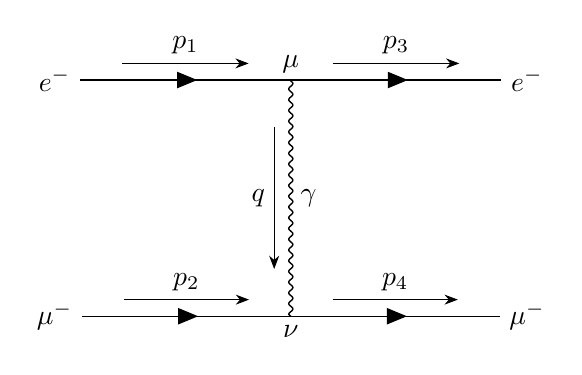
\begin{tikzpicture}[scale=2.0]
    \node at (0,-0.1) {$\nu$};
    \node at (0,1.6) {$\mu$};
    \begin{feynhand}
      % vertices
      \vertex (p11) at (1.5,0) {$\mu^-$};
      \vertex (p21) at (1.5,1.5) {$e^-$};
      \vertex (p12) at (-1.5,0) {$\mu^-$};
      \vertex (p22) at (-1.5,1.5) {$e^-$};
      \vertex (a) at (0,0); \vertex (b) at (0,1.5);
      % particles
      \propag [fer, mom=\(p_1\)] (p22) to (b);
      \propag [fer, mom=\(p_2\)] (p12) to (a);
      \propag [fer, mom=\(p_3\)] (b) to (p21);
      \propag [fer, mom=\(p_4\)] (a) to (p11);
      % exchange
      \propag [bos, mom'=\(q\)] (b) to [edge label=$\gamma$] (a);
    \end{feynhand}
  \end{tikzpicture}
  \caption{Diagram For Problem 3}\label{fig:p3}
\end{figure}
Using the Feynman rules, we can write each part as:
\begin{align*}
  -i\M&=\bar{u}(p_3)\qty[-ieQ_e\gamma^\mu]u(p_1)\\
  &\times -i\frac{g_{\mu\nu}}{q^2}\\
  &\times\bar{u}(p_4)\qty[-ieQ_\mu\gamma^\nu]u(p_2)
\end{align*}
From conservation of momentum, $q^2={(p_1-p_3)}^2=t$, we know that $Q_e=Q_\mu=-1$, and canceling out a few factors of $i$, we can find that:
\begin{align*}
  -i\M=i\frac{e^2}{q^2}\qty[\bar{u}(p_3)\gamma^\mu u(p_1)]
  g_{\mu\nu}
  \qty[\bar{u}(p_4)\gamma^\nu u(p_2)]
\end{align*}
Hence:
\begin{equation}
  \label{eq:p3a}
  \boxed{\M=-\frac{e^2}{{(p_1-p_3)}^2}\qty[\bar{u}(p_3)\gamma^\mu u(p_1)]
  g_{\mu\nu}\qty[\bar{u}(p_4)\gamma^\nu u(p_2)]}
\end{equation}
\begin{problem}
  \begin{enumerate}[label = (\alph*)]
    \setcounter{enumi}{1}
  \item Working in the center-of-mass frame, and writing $p^\mu_1=(E_1,0,0,p)$ and $p^\mu_3=(E_1,p\sin\theta,0,p\cos\theta)$, show that the electron currents for the four possible helicity combinations are:
    \begin{align*}
      \bar{u}_\downarrow(p_3)\gamma^\mu u_\downarrow(p_1)&=2(E_1c,ps,-ips,pc)\\
      \bar{u}_\uparrow(p_3)\gamma^\mu u_\downarrow(p_1)&=2(ms,0,0,0)\\
      \bar{u}_\uparrow(p_3)\gamma^\mu u_\uparrow(p_1)&=2(E_1c,ps,ips,pc)\\
      \bar{u}_\downarrow(p_3)\gamma^\mu u_\uparrow(p_1)&=-2(ms,0,0,0)
    \end{align*}
    Where $m$ is the electron mass, $s=\sin(\theta/2)$ and $c=\cos(\theta/2)$
  \end{enumerate}
\end{problem}
I just used Mathematica for this, notably, using the form of the spinors from the book with $\theta=0,\phi=0$ for $u(p_1)$, and $\theta=\theta,\phi=0$ for $u(p_3)$. The only additional step needed was to impose the condition that Mathematica did not have, mainly that $\vb{p}^2=p^2=E_1^2-m^2$, and we simply get the desired answer of:
\begin{equation}
  \label{eq:p3b}
  \boxed{
    \begin{aligned}
      \bar{u}_\downarrow(p_3)\gamma^\mu u_\downarrow(p_1)&=2(E_1c,ps,-ips,pc)\\
      \bar{u}_\uparrow(p_3)\gamma^\mu u_\downarrow(p_1)&=2(ms,0,0,0)\\
      \bar{u}_\uparrow(p_3)\gamma^\mu u_\uparrow(p_1)&=2(E_1c,ps,ips,pc)\\
      \bar{u}_\downarrow(p_3)\gamma^\mu u_\uparrow(p_1)&=-2(ms,0,0,0)
    \end{aligned}
  }
\end{equation}
See the attached Mathematica notebook for further details
\begin{problem}
  \begin{enumerate}[label = (\alph*)]
    \setcounter{enumi}{2}
  \item Explain why the effect of the parity operator $\hat{P}=\gamma^0$ is:
    \begin{align*}
      \hat{P}u_\uparrow(p,\theta,\phi)=
      u_\downarrow(p,\pi-\theta,\pi+\phi)
    \end{align*}
    Hence, or otherwise, show that the muon currents for the four helicity combinations are:
    \begin{align*}
      \bar{u}_\downarrow(p_4)\gamma^\mu u_\downarrow(p_2)&=2(E_2c,-ps,-ips,-pc)\\
      \bar{u}_\uparrow(p_4)\gamma^\mu u_\downarrow(p_2)  &=2(Ms,0,0,0)\\
      \bar{u}_\uparrow(p_4)\gamma^\mu u_\uparrow(p_2)    &=2(E_2c,-ps,ips,-pc)\\
      \bar{u}_\downarrow(p_4)\gamma^\mu u_\uparrow(p_2)  &=-2(Ms,0,0,0)
    \end{align*}
    Where $M$ is the muon mass
  \end{enumerate}
\end{problem}
The parity operator inverts all vector quantities (like momentum) yet maintains pseudo-vector quantities (like spin/helicity). In the spherical coordinates basis used in the book, this corresponds to the magnitude staying the same, and the $\theta$ angle being adjusted to $\pi-\theta$, and the $\phi$ angle being adjusted to $\phi+\pi$, hence:
\begin{align*}
  \hat{P}u_?(p,\theta,\phi)=u_?(p,\pi-\theta,\pi+\phi)
\end{align*}
what remains is the helicity. Since spin is a pseudo-vector, it is not inverted by parity, yet the \emph{helicity} still changes, as we have changed the direction of momentum, so instead of $\uparrow$, we invert it to $\downarrow$, giving the desired result
\begin{align*}
  \hat{P}u_\uparrow(p,\theta,\phi)=
  u_\downarrow(p,\pi-\theta,\pi+\phi)
\end{align*}
Now, we know that since we are working in the center of momentum frame, the muon momenta should be the parity inversion of the electron momenta, so we can write the muon spinors as:
\begin{align*}
  \hat{P}u_\uparrow(p_1)=u_\downarrow(p_4),\,\,
  \hat{P}u_\uparrow(p_3)=u_\downarrow(p_4),\,\,
  \hat{P}u_\downarrow(p_1)=u_\uparrow(p_4),\,\,
  \hat{P}u_\downarrow(p_3)=u_\uparrow(p_4)
\end{align*}
So we can write one of the muon currents in terms of the electron currents, sacrificing little generality:
\begin{align*}
  \bar{u}_{h_1}(p_4)\gamma^\mu u_{h_2}(p_2)&=
  \bar{(\hat{P}u_{\bar{h}_1}(p_3))}\gamma^\mu(\hat{P}u_{\bar{h}_2}(p_1))\\
  &={(\gamma^0u_{\bar{h}_1}(p_3))}^\dag
  \gamma^0\gamma^\mu\gamma^0u_{\bar{h}_2}(p_1)\\
  &=u^\dag_{\bar{h}_1}(p_3)\gamma^\mu\gamma^0u_{\bar{h}_2}(p_1)
\end{align*}
Using the anticommutator rules to swap the $\gamma^\mu$ and $\gamma^0$ leads to keeping the energy component the same and negating the spatial components, so in total we have to:
\begin{itemize}
\item Copy from electron spinor with BOTH helicities inverted
\item Keep energy component same sign
\item Flip sign of spatial components 
\end{itemize}
Hence the spinors have the following correspondence
\begin{align*}
  \bar{u}_\downarrow(p_4)\gamma^\mu u_\downarrow(p_2)\sim
  \bar{u}_\uparrow(p_3)\gamma^\mu u_\uparrow(p_1)\\
  \bar{u}_\uparrow(p_4)\gamma^\mu u_\downarrow(p_2)\sim
  \bar{u}_\downarrow(p_3)\gamma^\mu u_\uparrow(p_1)\\
  \bar{u}_\uparrow(p_4)\gamma^\mu u_\uparrow(p_2)\sim
  \bar{u}_\downarrow(p_3)\gamma^\mu u_\downarrow(p_1)\\
  \bar{u}_\downarrow(p_4)\gamma^\mu u_\uparrow(p_2)\sim
  \bar{u}_\uparrow(p_3)\gamma^\mu u_\downarrow(p_1)
\end{align*}
Giving the following muon currents
\begin{equation}
  \label{eq:p3c}
  \boxed{
    \begin{aligned}
      \bar{u}_\downarrow(p_4)\gamma^\mu u_\downarrow(p_2)&=2(E_2c,-ps,-ips,-pc)\\
      \bar{u}_\uparrow(p_4)\gamma^\mu u_\downarrow(p_2)&=-2(Ms,0,0,0)\\
      \bar{u}_\uparrow(p_4)\gamma^\mu u_\uparrow(p_2)&=2(E_2c,-ps,ips,-pc)\\
      \bar{u}_\downarrow(p_4)\gamma^\mu u_\uparrow(p_2)&=2(Ms,0,0,0)
    \end{aligned}
  }
\end{equation}
\newpage
\begin{problem}
  \begin{enumerate}[label = (\alph*)]
    \setcounter{enumi}{3}
  \item For the relativistic limit where $E\gg M$, show that the matrix element square for the case where the incoming $e^-$ and $\mu^-$ are both left-handed is given by:
    \begin{align*}
      \abs{\M_{LL}}^2=\frac{4e^4s^2}{{(p_1-p_3)}^4}
    \end{align*}
    Where $s={(p_1+p_2)}^2$. Fine the corresponding expressions for $\abs{M_{RL}}^2, \abs{M_{RR}}^2, \abs{M_{LR}}^2$
  \end{enumerate}
\end{problem}
In this limit, we ignore all the mass terms, and in each case $E=p$, where $E_1=E=E_2$. The only non-zero currents are:
\begin{align*}
  \bar{u}_\downarrow(p_3)\gamma^\mu u_\downarrow(p_1)&=2E(c,s,-is,c)\\
  \bar{u}_\uparrow(p_3)\gamma^\mu u_\uparrow(p_1)&=2E(c,s,is,c)\\
  \bar{u}_\downarrow(p_4)\gamma^\mu u_\downarrow(p_2)&=2E(c,-s,-is,-c)\\
  \bar{u}_\uparrow(p_4)\gamma^\mu u_\uparrow(p_2)&=2E(c,-s,is,-c)
\end{align*}
The matrix element $\M_{LL}$ corresponds to the situation where both currents are left handed, that is $\downarrow\downarrow$ for both muons and electrons. It may be valuable to compute all possible dot products now:
\begin{gather*}
  LL=j^e_{\downarrow\downarrow}\vdot j^\mu_{\downarrow\downarrow}
  =2E(c,s,-is,c)\vdot2E(c,-s,-is,-c)=4E^2(c^2+s^2+s^2+c^2)\\
  LR=j^e_{\downarrow\downarrow}\vdot j^\mu_{\uparrow\uparrow}
  =2E(c,s,-is,c)\vdot2E(c,-s,is,-c)=4E^2(c^2+s^2-s^2+c^2)
\end{gather*}
The remaining amplitudes should be the same, that is, $\abs{\M_{LR}}^2=\abs{\M_{RL}}^2$ and $\abs{\M_{LL}}^2=\abs{\M_{RR}}^2$. The matrix elements themselves are:
\begin{align*}
  \M_{LL}&=-\frac{e^2}{t}4E^2(c^2+s^2+s^2+c^2)=
  -\frac{e^2}{t}4E^2(1+1)=-\frac{e^2}{t}8E^2=-\frac{2se^2}{t}\\
  \M_{LR}&=-\frac{e^2}{t}4E^2(c^2+s^2-s^2+c^2)=
  -\frac{e^2}{t}4E^2(1+c^2-s^2)=-\frac{se^2}{t}(1+\cos\theta)
\end{align*}
Since we are in the center of mass frame, the energy $E=\sqrt{s}/2$. We can then write all of the squared amplitudes as:
\begin{equation}
  \label{eq:p3d}
  \boxed{
    \begin{aligned}
      \abs{\M_{LL}}^2&=\abs{\M_{RR}}^2=4e^4\frac{s^2}{t^2}\\
      \abs{\M_{LR}}^2&=\abs{\M_{RL}}^2=e^4\frac{s^2}{t^2}{(1+\cos\theta)}^2
    \end{aligned}
  }
\end{equation}
Where $t={(p_1-p_3)}^2$ for consistency with the problem statement
\begin{problem}
  \begin{enumerate}[label = (\alph*)]
    \setcounter{enumi}{4}
  \item In this relativistic limit, show that the differential cross section for unpolarized $e^-\mu^-\to e^-\mu^-$ scattering in the center-of-mass frame is:
    \begin{align*}
      \dv{\sigma}{\Omega}=\frac{2\alpha^2}{s}
      \frac{1+\frac14{(1+\cos\theta)}^2}{{(1-\cos\theta)}^2}
    \end{align*}
  \end{enumerate}
\end{problem}
We already calculated the spin-dependent matrix elements, so we can average them quite simply:
\begin{align*}
  \ev{\abs{\M}^2}&=\frac14
  \qty(\abs{\M}_{LL}^2+\abs{\M}_{LR}^2+\abs{\M}_{RL}^2+\abs{\M}_{RR}^2)\\
  &=\frac12\qty(\abs{\M}_{LL}^2+\abs{\M}_{RR}^2)\\
  &=2\frac{e^4s^2}{t^2}\qty(1+\frac14{(1+\cos\theta)}^2)
\end{align*}
First use the fact that $e^2=4\pi\alpha$ to write in terms of $\alpha$:
\begin{align*}
  \ev{\abs{\M}^2}=\frac{32\pi^2\alpha^2s^2}{t^2}
  \qty(1+\frac14{(1+\cos\theta)}^2)
\end{align*}
Since we are ignoring the masses, we can write $t$ in terms of $\theta$ and $s$:
\begin{align*}
  t&={(p_1-p_3)}^2=p_1^2+p_2^2-2p_1\vdot p_3
  =-2(E,0,0,E)\vdot(E,E\sin\theta,0,E\cos\theta)\\
  &=2E^2(1-\cos\theta)=\frac{s}2(1-\cos\theta)
\end{align*}
Giving us:
\begin{align*}
  \ev{\abs{\M}^2}&=\frac{128\pi^2\alpha^2s^2}{s^2{(1-\cos\theta)}^2}
  \qty(1+\frac14{(1+\cos\theta)}^2)\\
  &=\frac{128\pi^2\alpha^2}{{(1-\cos\theta)}^2}
  \qty(1+\frac14{(1+\cos\theta)}^2)
\end{align*}
The formula for the differential cross section is:
\begin{align*}
  \dv{\sigma}{\Omega}=\frac{1}{64\pi^2s}\frac{p_f^*}{p_i^*}\ev{\abs{\M}^2}
\end{align*}
Noting that momentum is conserved, the ratio will go away, leaving us with:
\begin{align*}
  \dv{\sigma}{\Omega}&=\frac{1}{64\pi^2s}
  \frac{128\pi^2\alpha^2}{{(1-\cos\theta)}^2}
  \qty(1+\frac14{(1+\cos\theta)}^2)\\
  &=2\frac{\alpha^2}{s}
  \frac{1+\frac14{(1+\cos\theta)}^2}{{(1-\cos\theta)}^2}
\end{align*}
Which is our final answer:
\begin{equation}
  \label{eq:p3e}
  \boxed{\dv{\sigma}{\Omega}=2\frac{\alpha^2}{s}
  \frac{1+\frac14{(1+\cos\theta)}^2}{{(1-\cos\theta)}^2}}
\end{equation}
\newpage
\section{Thomson, Problem 6.10}
\begin{problem}
  Use the trace formalism to calculate the QED spin-averaged matrix element squared for $e^+e^-\to f\bar{f}$ including the electron mass term.
\end{problem}
This is simply electron-positron annihilation, and since only fermions are involved, we only have the $s$-channel diagram as seen in figure~\ref{fig:p4}
\begin{figure}[H]
  \centering
  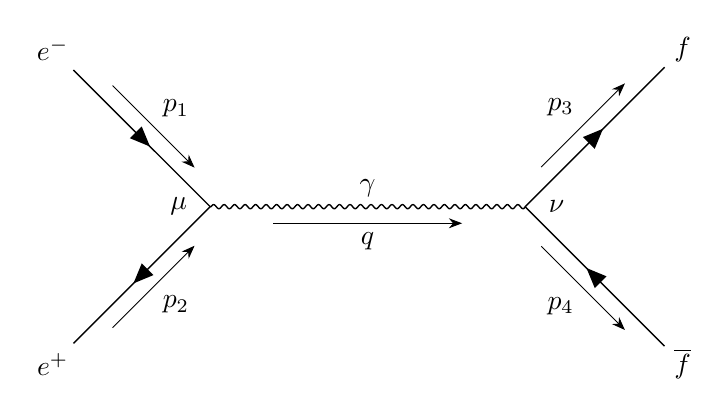
\begin{tikzpicture}[scale=2.0]
    \node at (-0.2,0) {$\mu$};
    \node at (2.2,0) {$\nu$};
    \begin{feynhand}
      % vertices
      \vertex (p11) at (-1,1) {$e^-$};
      \vertex (p12) at (-1,-1) {$e^+$};
      \vertex (p21) at (3,1) {$f$};
      \vertex (p22) at (3,-1) {$\bar{f}$};
      \vertex (a) at (0,0);
      \vertex (b) at (2,0);
      % particles
      \propag [fer, mom=\(p_1\)] (p11) to (a);
      \propag [antfer, mom'=\(p_2\)] (p12) to (a);
      \propag [fer, mom=\(p_3\)] (b) to (p21);
      \propag [antfer, mom'=\(p_4\)] (b) to (p22);
      % loop
      \propag [bos, mom'=\(q\)] (a) to [edge label=$\gamma$] (b);
    \end{feynhand}
  \end{tikzpicture}
  \caption{Diagram for Problem 4 representing $e^+e^-\to f\bar{f}$}\label{fig:p4}
\end{figure}
Notice this is identical to several calculations we have done so far, whether it be electron-positron annihilating to a muon-anti-muon pair or otherwise, the only difference is that we require a factor of $Q_f$ to stay rather than replacing it with the explicit value given, so it is sufficient to copy from say, eq (6.3) in the book, and inserting a factor of $Q_f$:
\begin{align*}
  \M=-\frac{Q_f e^2}{q^2}\qty[\bar{v}(p_2)\gamma^\mu u(p_1)]
  \qty[\bar{u}(p_3)\gamma_\mu v(p_4)]
\end{align*}
Squaring the matrix element:
\begin{align*}
  \M^*\M=\frac{Q_f^2e^4}{q^4}
  {\qty[\bar{v}(p_2)\gamma^\mu u(p_1)]}^*
  {\qty[\bar{u}(p_3)\gamma_\mu v(p_4)]}^*
  \qty[\bar{v}(p_2)\gamma^\nu u(p_1)]
  \qty[\bar{u}(p_3)\gamma_\nu v(p_4)]
\end{align*}
Summing over spins now allows us to write this as a trace over gamma matrices:
\begin{align*}
  \ev{\abs{\M}^2}=\frac{Q_f^2e^4}{4q^4}
  \Tr([\sla{p}_2-m_e]\gamma^\mu[\sla{p}_1+m_e]\gamma^\nu)
  \Tr([\sla{p}_3+m_f]\gamma_\mu[\sla{p}_4-m_f]\gamma_\nu)
\end{align*}
Consider the first trace, expand the product on the inside:
\begin{align*}
  [\sla{p}_2-m_e]\gamma^\mu[\sla{p}_1+m_e]\gamma^\nu=
  \sla{p}_2\gamma^\mu\sla{p}_1\gamma^\nu
  +m_e\sla{p}_2\gamma^\mu\gamma^\nu-m_e\gamma^\mu\sla{p}_1\gamma^\nu
  -m_e^2\gamma^\mu\gamma^\nu
\end{align*}
The inner terms, when written in terms of $\gamma$ matrices, contain an odd number of them, so their trace will be $0$:
\begin{align*}
  \Tr([\sla{p}_2-m_e]\gamma^\mu[\sla{p}_1+m_e]\gamma^\nu)
  =\Tr(\sla{p}_2\gamma^\mu\sla{p}_1\gamma^\nu-m_e^2\gamma^\mu\gamma^\nu)
\end{align*}
The second trace is quite simple:
\begin{align*}
  \Tr(-m_e^2\gamma^\mu\gamma^\nu)=-m_e^2\Tr(\gamma^\mu\gamma^\nu)
  =-4m_e^2g^{\mu\nu}
\end{align*}
The first one requires we unpack the slash notation:
\begin{align*}
  \Tr(\sla{p}_2\gamma^\mu\sla{p}_1\gamma^\nu)&=
  p_{2\sigma}p_{1\rho}\Tr(\gamma^\sigma\gamma^\mu\gamma^\rho\gamma^\nu)\\
  &=4p_{2\sigma}p_{1\rho}\qty(
  g^{\sigma\mu}g^{\rho\nu}+g^{\sigma\nu}g^{\mu\rho}-g^{\sigma\rho}g^{\mu\nu})\\
  &=4\qty(p_1^\nu p_2^\mu+p_1^\mu p_2^\nu-(p_1\vdot p_2)g^{\mu\nu})
\end{align*}
Leaving the total first trace as:
\begin{align*}
  \Tr([\sla{p}_2-m_e]\gamma^\mu[\sla{p}_1+m_e]\gamma^\nu)
  =4\qty(p_1^\nu p_2^\mu+p_1^\mu p_2^\nu-(p_1\vdot p_2)g^{\mu\nu}-m_e^2g^{\mu\nu})
\end{align*}
The second trace is essentially identical to this one, only with $p_3$ and $p_4$, lowered indices, and the fermion mass rather than $m_e$:
\begin{align*}
  \Tr([\sla{p}_3+m_f]\gamma_\mu[\sla{p}_4-m_f]\gamma_\nu)
  =4\qty(p_{3\nu} p_{4\mu}+p_{3\mu} p_{4\nu}
  -(p_3\vdot p_4)g_{\mu\nu}-m_e^2g_{\mu\nu})
\end{align*}
The term which appears in our spin-averaged matrix element is the product of these two terms:
\begin{gather*}
  \Tr([\sla{p}_2-m_e]\gamma^\mu[\sla{p}_1+m_e]\gamma^\nu)
  \Tr([\sla{p}_3+m_f]\gamma_\mu[\sla{p}_4-m_f]\gamma_\nu)\\
  =16\qty(p_1^\nu p_2^\mu+p_1^\mu p_2^\nu
  -(p_1\vdot p_2)g^{\mu\nu}-m_e^2g^{\mu\nu})
  \qty(p_{3\nu} p_{4\mu}+p_{3\mu} p_{4\nu}
  -(p_3\vdot p_4)g_{\mu\nu}-m_e^2g_{\mu\nu})\\
  \begin{aligned}
    =16&(
    {\color{red}(p_1\vdot p_3)(p_2\vdot p_4)}
    +{\color{green}(p_1\vdot p_4)(p_2\vdot p_3)}
    -{\color{blue}(p_1\vdot p_2)(p_3\vdot p_4)}\\
    &+{\color{green}(p_1\vdot p_4)(p_2\vdot p_3)}
    +{\color{red}(p_1\vdot p_3)(p_2\vdot p_4)}
    -{\color{blue}(p_1\vdot p_2)(p_3\vdot p_4)}\\
    &-{\color{blue}(p_1\vdot p_2)(p_3\vdot p_4)}
    -{\color{blue}(p_1\vdot p_2)(p_3\vdot p_4)}
    +{\color{blue}4(p_1\vdot p_2)(p_3\vdot p_4)}\\
    &+2m_f^2(p_1\vdot p_2)+2m_e^2(p_3\vdot p_4)+4m_e^2m_f^2
    )
  \end{aligned}
\end{gather*}
Note that all the blue terms cancel out, and the red and green terms combine to create:
\begin{gather*}
  \Tr([\sla{p}_2-m_e]\gamma^\mu[\sla{p}_1+m_e]\gamma^\nu)
  \Tr([\sla{p}_3+m_f]\gamma_\mu[\sla{p}_4-m_f]\gamma_\nu)\\
  =32[(p_1\vdot p_3)(p_2\vdot p_4)+(p_1\vdot p_4)(p_2\vdot p_3)
  +m_f^2(p_1\vdot p_2)+m_e^2(p_3\vdot p_4)
  +2m_e^2m_f^2
  ]
\end{gather*}
This diagram is $s$-channel, so the momentum transfer $q$ in the matrix element is $p_1+p_2$, so we end up with:
\begin{equation}
  \label{eq:p4}
  \boxed{
    \begin{aligned}
      \ev{\abs{\M}^2}=\frac{8Q_f^2e^4}{{(p_1+p_2)}^4}
      [&(p_1\vdot p_3)(p_2\vdot p_4)+(p_1\vdot p_4)(p_2\vdot p_3)\\
      &+m_f^2(p_1\vdot p_2)+m_e^2(p_3\vdot p_4)+2m_e^2m_f^2]
    \end{aligned}
  }
\end{equation}
\end{document}